\chapter{Subscript notation}
\label{ch:subnot1}


\section{Concept map}

Most of the discussion in the notes will assume a cartesian co-ordinate system unless otherwise mentioned.
You can read further about introduction to tensors in one of the following resources:
\begin{itemize}
\item Chapter 26 titled Tensors in~\cite{riley}.
\item The whole of ~\cite{bourne}.
\end{itemize}


\index{Concept map, subscript notation}

A concept map of how subscript notation will be used in this chapter is given in figure~\ref{subcmap}.
\begin{figure}[h]
 \centering
 \includegraphics[width=5 in]{images/c02-SubscriptConceptMap.eps}
 % ctrans.eps: 46x0 pixel, 300dpi, 0.39x0.00 cm, bb=0 35 595 420
 \caption{Concept map on the use of subscript notation in introducing tensors.}
 \label{subcmap}
\end{figure}



\section{Rules of subscript notation}

% learning objective
\begin{lo3}[Tensors]
Analyse free and dummy indices in an expression and determine number of components
\end{lo3}

Subscript notation \index{Subscript notation} was introduced by G. Ricci and popularised by Einstein. Each subscript (or index) runs from 1 to the dimension of the space in consideration. Since most of the time a 3D space is referred to, the subscripts run from 1 to 3. Following rules apply to the notation:

\begin{enumerate}
\item Cartesian Summation Convention: \index{Cartesian summation convention} Subscripts that are repeated are called dummy subscripts and should be summed over the range that the subscript can take. Dummy index should not appear more than twice in a term.
\item Subscripts that are not repeated are called free subscripts. 
\item Subscripts can come anywhere in an expression.
\item Subscripts after a comma indicate differentiation.
\item Free subscripts on either sides of the '$=$' sign should match. 
\end{enumerate} 

Subscript notation is useful to represent three and higher dimensional entities. It simplifies expressions.

{\bf Examples}
\begin{itemize}

\item Vector
$$ u_i = \left( u_1 \  u_2 \  u_3 \right) = \vec{u} = u_1 \hat{x}_1 + u_2 \hat{x}_2 + u_3 \hat{x}_3  $$

\item Matrices and Tensors
\begin{equation*}
a_{ij} = \left( \begin{array}{ccc}
a_{11} & a_{12} & a_{13} \\
a_{21} & a_{22} & a_{23} \\
a_{31} & a_{32} & a_{33} \\
\end{array}\right) 
\end{equation*} 

\item Nabla or Del or Grad:
\begin{equation*}
\vec{\nabla} =
\frac{\partial}{\partial x_1} \hat{x_1} +
\frac{\partial}{\partial x_2} \hat{x_2} +
\frac{\partial}{\partial x_3} \hat{x_3}
= \nabla_i
\end{equation*} 

\item Gradient:
\begin{equation*}
\vec{\nabla}\phi =
\frac{\partial \phi}{\partial x_1} \hat{x_1} +
\frac{\partial \phi}{\partial x_2} \hat{x_2} +
\frac{\partial \phi}{\partial x_3} \hat{x_3}
= \frac{\partial \phi}{\partial x_i} 
= \nabla_i\phi 
= \phi_{,i}
\end{equation*} 

\item Divergence:
$$ \vec{\nabla}\cdot\vec{u} = \frac{\partial u_1}{\partial x_1} + \frac{\partial u_2}{\partial x_2} + \frac{\partial u_3}{\partial x_3} $$
$$\text{Div}(u) = \frac{\partial u_i}{\partial x_i} = u_{i,i} $$

\item Inner product \index{Inner product} is an operation where there is a contraction of the number of subscripts. For two vectors, it is also called as dot product.
$$a_{i}b_{i} = a_1b_1 + a_2b_2 + a_3b_3 $$

$$ a_{i}a_{i} = a_1^2 + a_2^2 + a_3^2 $$

\begin{equation*}
\begin{array}{c}
c_j = a_{ij}b_{i} \\
c_1 = a_{11}b_1 + a_{21}b_2 + a_{31}b_3\\
\vdots
\end{array}
\end{equation*} 


\item Outer product \index{Outer product} is an operation where there is a an expansion of the number of subscripts.
\begin{equation*}
a_{i}b_{j} = \left( \begin{array}{ccc}
a_{1}b_{1} & a_{1}b_{2} & a_{1}b_{3} \\
a_{2}b_{1} & a_{2}b_{2} & a_{2}b_{3} \\
a_{3}b_{1} & a_{3}b_{2} & a_{3}b_{3} \\
\end{array}\right) 
\end{equation*} 

\end{itemize}

% ----------------------------------------------------------------------------

\begin{question}
Subscripts that are not repeated are called free subscripts. Each subscript (or index) runs from 1 to the dimension of the space (3, by default). 
Fill the number of components for each of the following quantities.
	\begin{enumerate}
		\item $u_i$
		\item $\sigma_{ij}$
		\item $\epsilon_{ijk}$
		\item $\mu_{ijkl}$
	\end{enumerate}

Think of these entities as those physical parameters that can be represented by a bunch of numbers in any given coordinate system. These numbers can be arranged as matrices for convenience.
\end{question}
\begin{solution}[print]
	\begin{enumerate}
		\item $u_i$ : $3^1=3$
		\item $\sigma_{ij}$ : $3^2=9$
		\item $\epsilon_{ijk}$ : $3^3=27$
		\item $\mu_{ijkl}$ : $3^4=81$
	\end{enumerate}
\end{solution}

% ----------------------------------------------------------------------

\begin{question}
Cartesian summation convention: Subscripts that are repeated are called dummy subscripts and should be summed over the range that the subscript can take. The rest of the subscripts are free subscripts. 
Fill the number of components for each of the following quantities.

	\begin{enumerate}
		\item $u_i v_i$ 
		\item $a_{ij} b_{ij}$ 
		\item $d_{ijk} E_k$ 
		\item $\epsilon_{ijk} \sigma_{ij}$ 
		\item $S_{ijkl} \sigma_{kl}$ 
		\item ${1 \over 2} C_{ijkl} e_{ij} e_{kl}$ 
		\item $\chi_{ijkl} E_{j} E_{k} E_{l}$ 
	\end{enumerate}
\end{question}
\begin{solution}[print]
	\begin{enumerate}
		\item $u_i v_i$ : $3^0=1$
		\item $a_{ij} b_{ij}$ : $3^0=1$
		\item $d_{ijk} E_k$ : $3^2=9$
		\item $\epsilon_{ijk} \sigma_{ij}$ : $3^1=3$
		\item $S_{ijkl} \sigma_{kl}$ : $3^2=9$
		\item ${1 \over 2} C_{ijkl} e_{ij} e_{kl}$ : $3^0=1$
		\item $\chi_{ijkl} E_{j} E_{k} E_{l}$ : $3^1=3$
	\end{enumerate}
\end{solution}

% ----------------------------------------------------------------------

\begin{question}
Subscripts can come anywhere in an expression.
Fill the number of components for each of the following quantities.
	\begin{enumerate}
		\item $\partial u_i \over \partial x_i$
		\item $\partial \sigma_{ij} \over \partial x_j$
		\item $\partial u_i \over \partial x_j$
		\item $\rho_{mn} J_n + \alpha_{mn} {\partial T \over \partial Z_n}$
	\end{enumerate}
\end{question}
\begin{solution}[print]
	\begin{enumerate}
		\item $\partial u_i \over \partial x_i$ : $3^0=1$
		\item $\partial \sigma_{ij} \over \partial x_j$ : $3^1=3$
		\item $\partial u_i \over \partial x_j$ : $3^2=9$
		\item $\rho_{mn} J_n + \alpha_{mn} {\partial T \over \partial Z_n}$ : $3^1=3$
	\end{enumerate}
\end{solution}

% ----------------------------------------------------------------------

\begin{question}
Subscripts after a comma indicate differentiation.
$$ u_{i,i} = {\partial u_i \over \partial x_i} = {\partial u_1 \over \partial x_1} + {\partial u_2 \over \partial x_2} + {\partial u_3 \over \partial x_3} $$

	\begin{enumerate}
		\item $\sigma_{ij,j}$
		\item $u_{i,j}$
	\end{enumerate}
\end{question}
\begin{solution}[print]
	\begin{enumerate}
		\item $\sigma_{ij,j}$ : ${\partial \sigma_{i1} \over \partial x_1} + {\partial \sigma_{i2} \over \partial x_2} + {\partial \sigma_{i3} \over \partial x_3}$ 
		\item $u_{i,j}$ : A matrix of 9 elements
	\end{enumerate}
\end{solution}

% ----------------------------------------------------------------------

% learning objective
\begin{lo2}[Tensors]
\label{lo2.1}
Validate an expression to be conforming to the rules of subscript notation
\end{lo2}

% ----------------------------------------------------------------------

\begin{question}
Free subscripts on either sides of the '$=$' sign should match. In an expression, each term shall have the same free subscript.
	Identify the errors in the following expressions. [LO~\ref{lo2.1}]
	\SetQuestionProperties{
		LearningObjectives = \ref{lo2.1},
		}
	\begin{enumerate}
		\item $a_i = {\partial u_i \over \partial x_i} + b_j $
		\item $J_i = -k_{ij}{\partial T \over \partial x_j} + q_j$
		\item ${\partial u_i \over \partial t} + u_j {\partial u_i \over \partial x_j} = - {\partial p \over \partial x_i} + F_j $
	\end{enumerate}
\end{question}
\begin{solution}[print]
	Corrected expressions are given as follows:
	\begin{enumerate}
		\item $a_{ij} = {\partial u_i \over \partial x_j} + b_{ij} $
		\item $J_i = -k_{ij}{\partial T \over \partial x_j} + q_i$
		\item ${\partial u_i \over \partial t} + u_j {\partial u_i \over \partial x_j} = - {\partial p \over \partial x_i} + F_i $ 
	\end{enumerate}
\end{solution}

% ----------------------------------------------------------------------

\section{Nabla}

{\bf Nabla or Del or Grad}
\begin{equation*}
\vec{\nabla} =
\frac{\partial}{\partial x_1} \hat{x_1} +
\frac{\partial}{\partial x_2} \hat{x_2} +
\frac{\partial}{\partial x_3} \hat{x_3}
= \nabla_i
\end{equation*} 

% ------------------------------------------------------------------
\begin{question}
Write the following using the above convention.
	\begin{enumerate}
		\item Gradient of a scalar function $\phi$
		\item Divergence of a vector $\vec{u}$
	\end{enumerate}
\end{question}
\begin{solution}[print]
	\begin{enumerate}
		\item Gradient of a scalar function $\phi$ is $\nabla_i \phi$
		\item Divergence of a vector $\vec{u}$ is $\nabla_i u_j \delta_{ij} = \nabla_i u_i$
	\end{enumerate}
\end{solution}
% ------------------------------------------------------------------

\section{Kronecker Delta}

% learning objective
\begin{lo3}[Preliminaries]
Apply the definition of Kronecker delta to simplify expressions in subscript notation
\end{lo3}

Definition of Kronecker delta \index{Kronecker delta} which is used to represent an isotropic tensor of order 2 is : 
$$ \delta_{ij} = 
\begin{array}{lll}
1 & \mathrm{if} & i=j \\
0 & \mathrm{if} & i \ne j\\
\end{array} $$

\begin{equation*}
\delta_{ij} = \left( \begin{array}{ccc}
1 & 0 & 0 \\
0 & 1 & 0 \\
0 & 0 & 1 \\
\end{array}\right) 
\end{equation*} 

\begin{itemize}
\item Trace of a matrix $a$
$$ \text{Tr}(a) = a_{ij}\delta_{ij} = a_{ii} = a_{11}+a_{22}+a_{33}$$
$$\boxed{ \text{Tr}(a) = a_{ii} }$$

\item Trace of $\delta_{ij}$ is $\delta_{ii}=3$.

\item $\delta_{ij}$ is used to simplify expressions involving dummy indices.
Consider $b_{ik} = a_{ij} \delta_{jk}$ Expand the expression for a given $i,k$ and convince yourself that 
$$ \boxed{a_{ik} \delta_{ij} = a_{jk} }$$
$$p_i \delta_{ij} = p_j$$
\end{itemize}

% -----------------------------------------------

\begin{question}
Evaluate the following and comment.

	\begin{enumerate}
		\item $a_i b_j \delta_{ij}$
		\item $a_i b_i$
		\item $c_{ij} \delta_{ij}$
		\item $\delta_{ij} \delta_{ij}$
	\end{enumerate}
\end{question}
\begin{solution}[print]
	\begin{enumerate}
		\item $a_i b_j \delta_{ij}$ = $a_1 b_1 + a_2 b_2 + a_3 b_3$
		\item $a_i b_i$ = $a_1 b_1 + a_2 b_2 + a_3 b_3$
		\item $c_{ij} \delta_{ij}$ = $c_{11} + c_{22} + c_{33}$
		\item $\delta_{ij} \delta_{ij}$ = $3$
	\end{enumerate}
\end{solution}


% -----------------------------------------------

\begin{question}[ID=kdelteuse1]
From the above expressions, can you discover what the Kronecker delta would do to one of the matching indices?
\end{question}
\begin{solution}[print]
Identify a term that is summed with Kronecker delta over one of the indices. Replace that index in the term with the free index of Kronecker delta. See for example:
$$ a_{ik} \delta_{ij} = a_{jk}$$
\end{solution}

% -----------------------------------------------
% learning objective
\begin{lo3}[Preliminaries]
Apply the definition of Levi-Civita symbol to simplify expressions in subscript notation
\end{lo3}


\section{Levi-Civita Symbol}

Levi-Civita symbol is also called as permutation matrix or alternator. \index{Permutation matrix} \index{Levi-Civita symbol}

Definition: 
$$ \epsilon_{ijk} = 
\begin{array}{ll}
1 & \mathrm{if}\  i,j,k \  \mathrm{appear \  cyclic} \\
-1 & \mathrm{if}\  i,j,k \  \mathrm{donot \ appear\ cyclic} \\
0 & \mathrm{if}\ i=j \  \mathrm{or} \  j=k \ \mathrm{or} \  k=i  \\
\end{array} $$

$$ 
\begin{array}{l}
\epsilon_{123} = \epsilon_{231} = \epsilon_{312} = 1 \\
\epsilon_{132} = \epsilon_{213} = \epsilon_{321} = -1 \\
\epsilon_{111} = \epsilon_{112} = \epsilon_{211} =\epsilon_{121} = \epsilon_{113} = \epsilon_{311} =\epsilon_{131} = 0 \\
\epsilon_{222} = \epsilon_{221} = \epsilon_{122} =\epsilon_{212} = \epsilon_{223} = \epsilon_{322} =\epsilon_{232} = 0 \\
\epsilon_{333} = \epsilon_{331} = \epsilon_{133} =\epsilon_{313} = \epsilon_{332} = \epsilon_{233} = \epsilon_{323} = 0 \\
\end{array}
$$

Permutation matrix will help in writing expressions involving a cross product in a simplified manner.

One can write $\epsilon_{ijk}$ also in terms of a triple product as follows:

$$ \epsilon_{ijk} = \left[ \hat{x_i}, \hat{x_j}, \hat{x_k} \right] $$

% ---------------------------------------------------------------

\begin{question}
What is the value of $\epsilon_{ijk} \epsilon_{ijk}$ ?
\end{question}
\begin{solution}[print]
6
\end{solution}

% ---------------------------------------------------------------


Expand the following expressions separately and write in the box what they usually mean.


\begin{tabular}{| c | m{4cm} | m{5 cm} |}
\hline
Expression & No. of components & Comment \\
\hline
$\epsilon_{ijk} u_j v_k$ & &\\[1cm]
\hline
$\epsilon_{ijk} u_{k,j}$ &  & \\[1cm]
\hline
$\epsilon_{ijk} a_{1i} a_{2j} a_{3k}$ &  & \\[1cm]
\hline
\end{tabular}

% -----------------------------------------------------------------
% learning objective
\begin{lo3}[Preliminaries]
Convert an expression in vectorial notation to subscript notation
\end{lo3}

% -----------------------------------------------------------------

% learning objective
{\bf Utility of permutation matrix}:

If you have discovered the utility of $\epsilon_{ijk}$ to write cross products, then write the following expressions in their equivalent subscript notation.

\begin{tabular}{| c | m{2cm} | m{7 cm} |}
\hline
Vectorial Expression & free index & expression in subscript notation \\
\hline
$\vec{c} = \vec{a} \times \vec{b}$ & &\\[1cm]
\hline
$\vec{c} = \vec{\nabla} \times \vec{a}$ & &\\[1cm]
\hline
$\vec{c} \cdot \left( \vec{\nabla} \times \vec{a} \right)$ & &\\[1cm]
\hline
$\vec{c} \times \left( \vec{\nabla} \times \vec{a} \right)$ & &\\[1cm]
\hline
\end{tabular}


Discuss with your neighbour and answer the following.


\begin{enumerate}
\item In what kind of vectorial expressions do you need to know how to simplify terms where the permutation matrix appears twice.

\item Within a term written using subscript notation, is the sequence of the terms important? If no - why? If yes - in what situations.

\end{enumerate}

\begin{itemize}

\item Curl :
$$ \vec{p} = \vec{\nabla}\times\vec{u}$$
$$ p_i = \epsilon_{ijk} \nabla_j u_k = \epsilon_{ijk} u_{k,j} = \epsilon_{ijk} \frac{\partial u_k}{\partial x_j}$$
$$\boxed{ \text{Curl}(u) = \epsilon_{ijk} \frac{\partial u_k}{\partial x_j} }$$

\item Cross Product : \index{Cross product}
$$ \vec{p} = \vec{u}\times\vec{v}$$
$$ \boxed{p_i = \epsilon_{ijk} u_j v_k }$$

\item Condition for coplanarity of three vectors $a_i$, $b_j$ and $c_k$ is:
$$ \epsilon_{ijk} a_i b_j c_k = 0 $$
\index{Determinant}
\item Determinant of a matrix $a$ : 
$$\text{Det}(a) = \| a_{ij} \|$$
$$ \boxed{\text{Det}(a) = \epsilon_{ijk}a_{1i}a_{2j}a_{3k}} $$

\end{itemize}

% ---------------------------------------------------------------

\section{Summary}
\begin{enumerate}
\item Kronecker delta $\delta_{ij}$ and its application to dot product.
\item Levi-Civita symbol $\epsilon_{ijk}$ and its application to cross product.
\end{enumerate}

% ---------------------------------------------------------------

